\section{Abstract}

The World Wide Lightning Location Network (WWLLN) is a long range network capable of locating lightning strokes in space and time.
While able to locate lightning to within a few kilometers and ten microseconds, the network currently does not measure any characteristics of the strokes themselves.
The capabilities of the network are expanded to allow for measurements of the far-field power from the root mean square electric field of the detected strokes in the 6-18~kHz band.
This is accomplished by calibrating the network from a single well calibrated station using a bootstrapping method.
With this technique the global median stroke power seen by the network is 1.0 x $10^6$~watts with an average uncertainty of 17\%.
The results are validated by comparing to return stroke peak current as measured by the New Zealand Lightning Detection Network and to previous ground wave power measurements in the literature.
Our global median stroke power is found to be four orders of magnitude lower than reported earlier for the measurements including the nearby ground and sky wave.
However, we find our far-field waveguide mode observations are consistent with the previous literature due to differences in observational techniques and the efficiency of coupling into a propagation wave in the Earth-ionosphere waveguide.
This study demonstrates that the WWLLN determined powers can be used to estimate the return stroke peak currents of individual lightning strokes occurring throughout the globe.

\section{Introduction}

The World Wide Lightning Location Network (WWLLN, see http://wwlln.net) determines the location for nearly all lightning producing storms around the globe in real time (c.f. \citet{Jacobson2006c}).
The network uses Very Low Frequency (VLF) radio wave receivers distributed around the globe to identify the time of group arrival (TOGA) for the wave packets of individual lightning sferics \citep{Dowden2002d}, and a central processor combines the TOGAs to determine the source locations over the spherical Earth.
Knowledge of individual stroke locations, with high temporal accuracy, and within a fraction of a wavelength is beneficial for both scientific and technical uses. WWLLN lightning location data have recently been used for advances in space science (c.f. \citet{Kumar2009}, or \citet{Holzworth2011}), meteorology (c.f. \citet{Price2009}, \citet{Thomas2010d}) and detailed lightning physics (\citet{Connaughton2010a}) to name a few.
Near instantaneous knowledge of lightning stroke location anywhere in the world, provided by WWLLN, is now actively used by the USGS (U.S. Geological Survey) to help identify remote, explosive volcanic eruptions (see \citet{Doughton2010}).

WWLLN currently consists of 57 VLF stations distributed as shown in figure~\ref{energy:fig:wwlln_dist}, with more stations continuously being added to the network.
As stations are added the accuracy and detection efficiency of the network improves. As of 2010 the network locates most strokes to within 10 kilometers and $<$10~$\mu$s with an estimated detection efficiency of about 11\% for all strokes and $>$30\% for more powerful strokes \citep{Abarca2010,Rodger2009}.
The network uses a TOGA technique, originally developed by \citet{Dowden2000}, to locate strokes by analyzing the sferic waveforms at each station using the Stroke\_B algorithm as discussed by \citet{Rodger2006,Rodger2009}.

 \begin{figure}[b]
 \noindent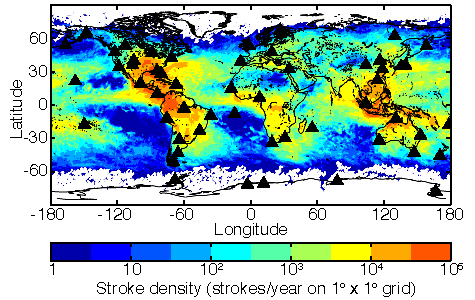
\includegraphics[width=19pc,angle=0]{energy/Figures/PPS_WWLLN_2010.pdf}\\
 \caption{WWLLN 2010 global stroke density on $1^\circ$ x $1^\circ$ grid, station locations shown with black triangles. Data processed with the Stroke\_B algorithm.}
 \label{energy:fig:wwlln_dist}
 \end{figure}

As only the spectral variations through the sferic wave packet are needed for determining the TOGA, the absolute electric field amplitude is unnecessary to accurately locate lightning. Due to this, the network does not currently report other characteristics of strokes such as peak current.
However, each WWLLN station does record the root mean square (RMS) electric field value of the sferic waveform used in the TOGA calculation, but these values need to be calibrated, as discussed below.

The station operated by the University of Otago near New Zealand's Antarctic station, Scott Base, was calibrated by a field team in December 2009.
The field team injected a series of calibration signals, ramped progressively in frequency, through the crossed magnetic loops of the Scott Base antenna and computed the calibration from the equivalent electric field.
This calibration of a single station allows for the calculation of stroke power as seen by the network.

A previous study by \citet{Rodger2006} attempted to calibrate the network through observations of narrow-band VLF communication transmitters at each WWLLN station.
These observations were combined with the U.S. Navy Long Wave Propagation Capability (LWPC) code, described by \citet{Ferguson1998}, to predict what the received amplitude should be in order to calibrate each station.
However the study assumed that the frequency response of the sound cards was the same across the network, an assumption which was false.
The current study utilizes a broader range of frequencies and calibrates each station such that differing frequency responses are accounted for in the calibration.

Measuring stroke power is an important step forward as it allows the network to make real time measurements of the strength of lightning worldwide.
Being able to measure characteristics of the strokes will allow for insights into thunderstorm evolution, large scale storm phenomena, and global effects of lightning.
For example, stroke power values could help current research on terrestrial gamma ray flashes by \citet{Briggs2011} constraining efficiencies and source mechanisms, and tropical hurricanes by \citet{Thomas2010d} could utilize the power in analyzing eyewall replacement.

As we will show here, the network measures a median global VLF stroke power in the far-field waveguide mode of 1.0 x $10^6$~W with an average uncertainty of 17\%.
Previous measurements have shown the power radiated by strokes is often near $10^{10}$~W \citep{Krider1983}. This difference is due to methodology in the measurements.
Past measurements used a broad band peak power measurement taken in range of the ground wave (100~km), while WWLLN measures the power in the 6-18~kHz band from the RMS electric field at much longer distances.
When these factors are accounted for the median power from WWLLN located strokes is comparable to the previously reported value of $10^{10}$~W peak power.

\section{Instrumentation and Data Processing}

In order to calculate the stroke power from WWLLN three steps are necessary: measure RMS electric field of a stroke, calculate the stroke power needed to produce the electric field at the station, and calibrate each station in the network.

\subsection{Station Electric Field}

Each WWLLN station consists of four main components: the antenna, a preamplifier, a service unit for signal and power management, and the sound card that digitizes the measured fields.
The difficulty in making a power measurement with the network arises in calibrating for the coupling between a short (2m) station antenna to a signal with an approximately $\sim$10~km wavelength.
When a station digitizes the electric field waveform it stores it in uncalibrated sound card units (SCU).
Additionally, the effective gain and calibration differs at each station due to the preamplifier, antenna construction, soundcard frequency response, and local environmental conditions.
This results in the RMS electric field being reported in station specific sound card units.

The average power spectra from 194 stroke waveforms recorded at the Tallahassee, Florida station are shown in figure~\ref{energy:fig:average_spectra} along with the frequency response of a typical preamplifier.
The strokes used were located at distances of 5000~km to 10000~km from the station and were recorded between 18:00 and 21:00 UTC on May 3 and May 9 2011.
As can be seen in the figure the power peaks between 6-18 kHz with the analog response remaining relatively flat through the entire frequency range.
The spikes in the power spectra are a result of manmade VLF communication transmitters.

 
 \begin{figure}[t]
 \noindent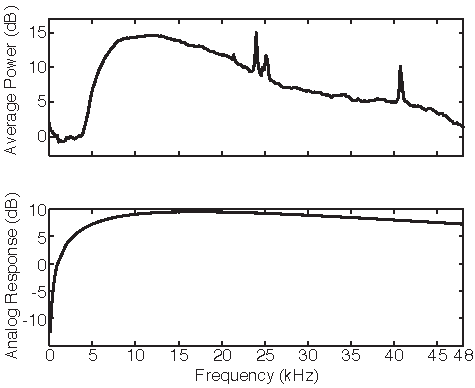
\includegraphics[width=19pc,angle=0]{energy/Figures/PPS_Spectra.pdf}\\
 \caption{The top panel shows average power spectra from 194 stroke waveforms recorded at the Tallahassee, FL station between 0 and 48 kHz. The strokes were located between 5000km and 10000km away from the  station on May 3 2011 and May 9 2011 between 18:00 and 21:00 UTC. The bottom panel shows the frequency response of the preamplifier.}
 \label{energy:fig:average_spectra}
 \end{figure}

The waveforms used are 1.33 ms long with 0.33 ms pre-trigger and 1 ms post-trigger.
Prior to processing the waveform is put through a 6-18~kHz 16 point finite impulse response (FIR) bandpass filter.
The RMS value of the resultant waveform is stored in uncalibrated sound card units.
After being calibrated to the $\sim$10~km wavelength signal the SCU measurement can be converted into the RMS electric field of the sferic. 

\subsection{LWPC and Power}

To calculate the stroke power based on the RMS electric field at a station the LWPC code is used to model the attenuation, as a function of frequency, between a transmitter at the stroke location and the receiving station.
The LWPC code was developed by the Space and Naval Warfare Systems Center by \citet{Ferguson1998} and has most recently been validated by \citet{Thomson2011}.
In this research we made use of LWPC version 2.1.

With a known conversion from a stations SCU value to V m$^{-1}$, $A_{local}$, of the lightning waveform, power is calculated using equation~\ref{energy:eq:power_eq}.
The ratio from LWPC between a 100kW transmitter and the modeled field (given in dB above 1 $\mu$V m$^{-1}$) is used to account for the sferic attenuation, $\alpha$, along the path for every grid location for every detector.

\begin{equation}
P_{stroke}=\frac{E_{scu}^2}{A_{local}^2} * \frac{100kW}{(10^{\alpha/20}\mu V/m)^2}
\label{energy:eq:power_eq}
\end{equation}

Since energy of the stroke is the time integrated electric field, and the power measurements are from the RMS electric field value, the energy of the stroke can be found from the size of the triggering window: $E_{stroke}=P_{stroke} * t_{window}$, with the current triggering window set at 1.33 ms.

Due to computing limitations running the LWPC code, we cannot conduct a full run for every stroke-station pair in real time.
Instead a lookup table is used which breaks stroke locations into $5^{\circ}$ by $5^{\circ}$ bins and uses either an all day ($\beta=0.3$ km$^{-1}$ and $h'=74$ km) or an all night ($\beta(f)=0.3-0.8$ km$^{-1}$ and $h'=87$ km) ionospheric model, where $\beta$ and $h'$ are the slope of the conductivity ($\beta$ is frequency dependent at night) and the reference height in the ionospheric model.
The ionospheric models are the default models of LWPC code and fully described in \citet{Ferguson1998}. 
To account for transitions across the terminator a weighted average of the day and night electric field values are used.
The lookup tables give the electric field averaged over the 8 - 18 kHz band which captures the frequencies of the peak radiated power from lightning (6-7 kHz omitted due to code limitations) \citep{Volland1995}.
An example of the day ionosphere lookup table for the Dunedin station is shown in figure~\ref{energy:fig:lookup}.
The discontinuity of electric field over Greenland and in the South Atlantic is caused by the high attenuation rate of VLF propagating over ice.

 \begin{figure}[t]
 \noindent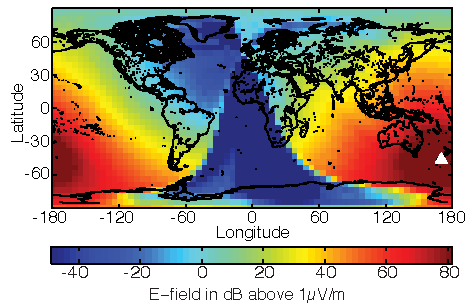
\includegraphics[width=19pc,angle=0]{energy/Figures/PPS_Lookup.pdf}\\
 \caption{LWPC generated lookup table for Dunedin station (white triangle) using an all day ionospheric model ($\beta=0.3$ km$^{-1}$ and $h'=74$ km) averaged over 8-18 kHz. Each $5^{\circ}$ by $5^{\circ}$ bin shows the electric field seen at Dunedin if a 100kW transmitter is centered on that bin.}
 \label{energy:fig:lookup}
 \end{figure}

\subsection{Calibration and Bootstrapping}

With one calibrated station it is possible to find the calibration of other nearby stations.
The process is shown in figure~\ref{energy:fig:calibrate}.
Using a well calibrated station (on the right) the stroke power of a given stroke is found using LWPC for the same stroke.
The uncalibrated station also finds the power using LWPC, however instead of a power in watts, it measures the power in sound card power, SCP.
The ratio between the two power values will give the calibration factor, $A_{local}^2$, of the second station.
This is repeated for many strokes with the median of the conversion factor distribution used as the conversion factor between the two stations.

\begin{figure}[t]
\noindent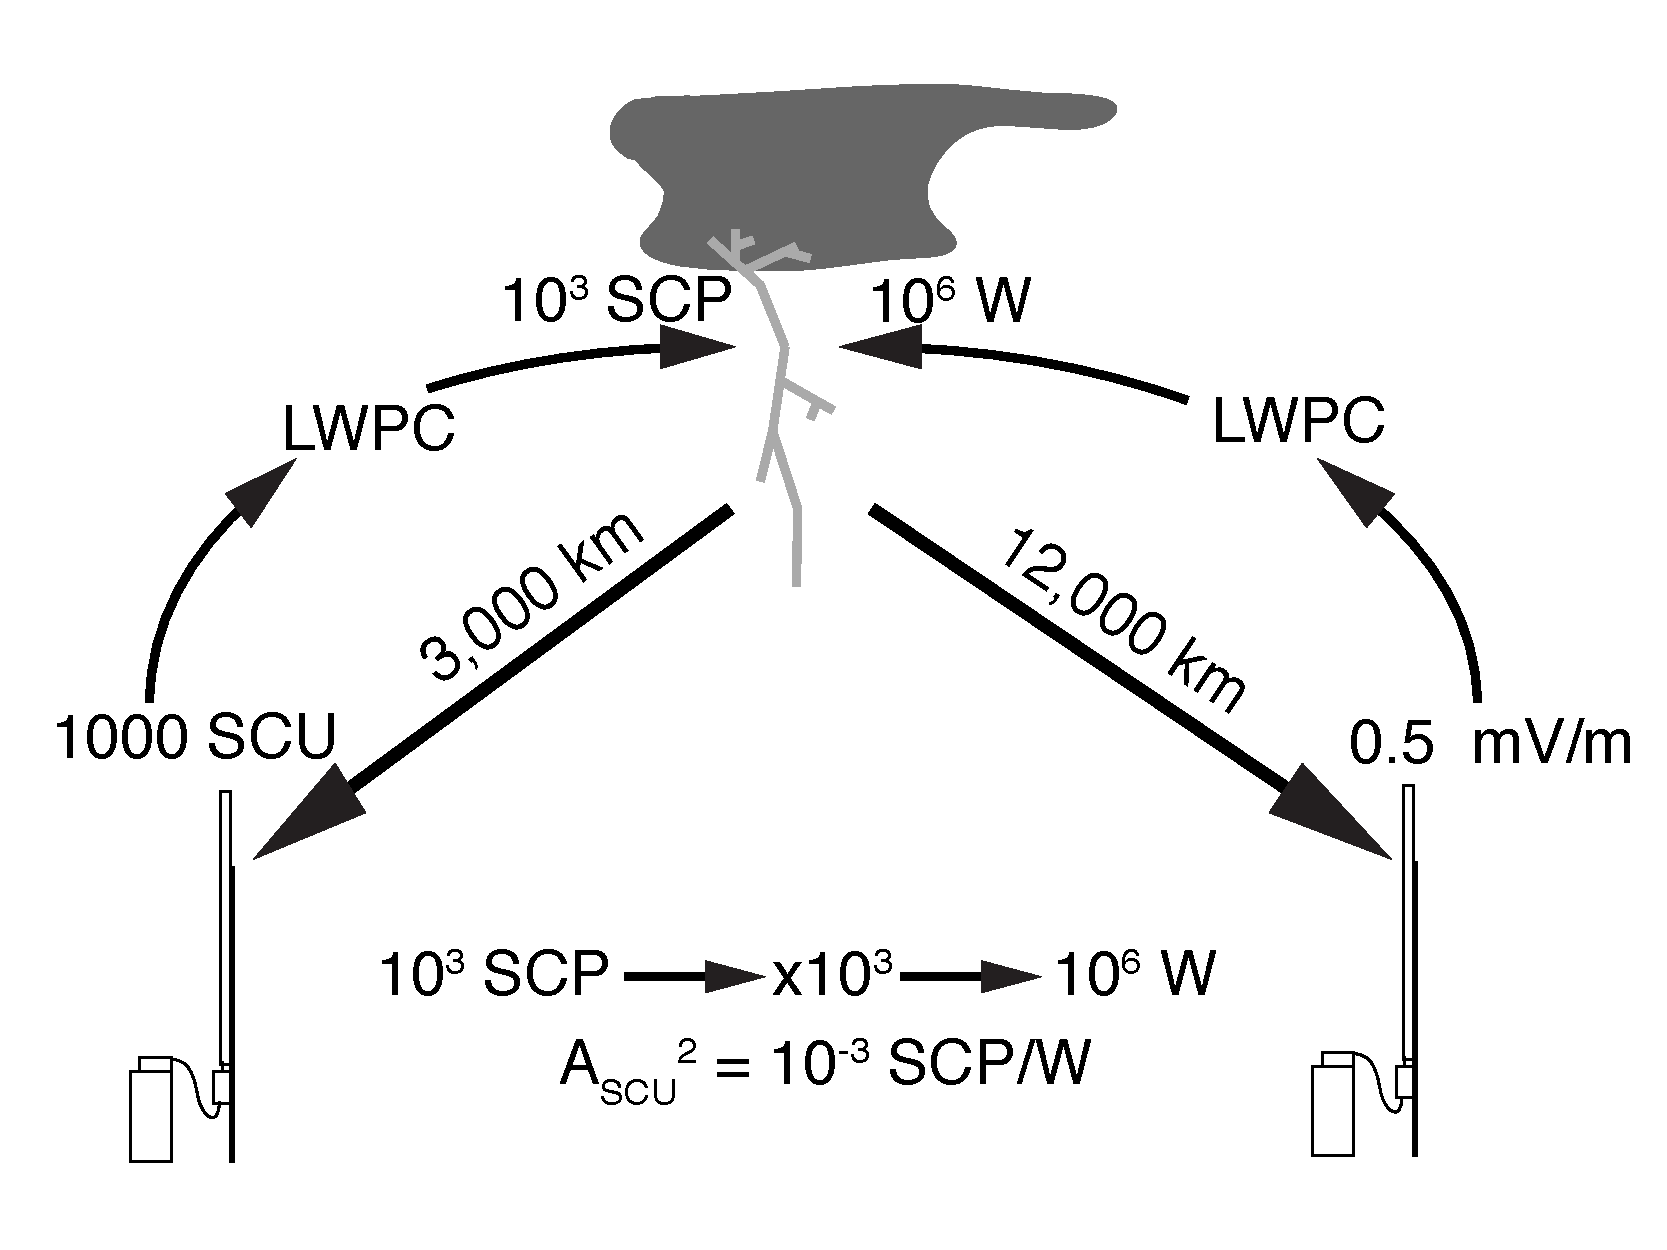
\includegraphics[width=19pc,angle=0]{energy/Figures/PPS_Method.pdf}\\
\caption{Method of calibrating one station to another using LWPC.}
\label{energy:fig:calibrate}
\end{figure}

Only one station in the network is thoroughly calibrated to VLF fields, the station in Scott Base, Antarctica.
Using the method described below the Dunedin station was calibrated off of Scott Base station.
With both stations calibrated, Dunedin was chosen as the first calibrated station in the bootstrapping process, by using thousands of mutually observed sferics.
Dunedin was chosen instead of Scott Base due to strong observed seasonal variations likely due to changes local ground conductivity that are not accounted for in the propagation model.

To calibrate the entire network off of a single station a bootstrapping method is used.
Station to station calibrations are done using strokes that have all day paths to both stations and are within 1000-8000 km of both stations.
All day paths were chosen as the daytime ionosphere is modeled more accurately by LWPC than the night ionosphere \citep{McRae2000d}.

The first set of calibrations are done between the well calibrated station and those with common strokes that have the desired path characteristics.
Once calibrated these stations are used to calibrate the next set of stations, and these newly calibrated stations are used to find the next set.
This process is repeated until no further stations can be calibrated, figure~\ref{energy:fig:bootstrap} is an example of this process.
Not all stations are calibrated for each day, they may not be calibrated if they do not see any common strokes with another station that match the path requirements or if their calibration to the next set of stations does not match direct calibrations.
For example, if station A calibrates B and then B calibrates C then if the calibration path ABC does not match the well calibrated path of AC it is determined that B is not well calibrated, so it is not used.

 \begin{figure}[t]
 \noindent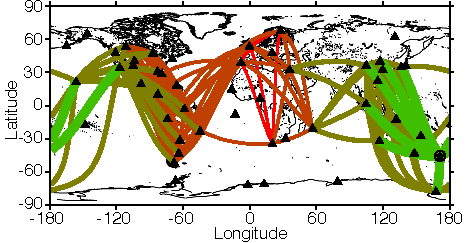
\includegraphics[width=19pc,angle=0]{energy/Figures/PPS_Hop.pdf}\\
 \caption{An example of the bootstrapping technique, showing calibration distance from the main Dunedin station. Thick green lines are the first calibration stage and the thin red lines the last. Stations may be unconnected due to not having common strokes, being poor intermediary stations or being down for the day.}
 \label{energy:fig:bootstrap}
 \end{figure}

\subsection{Power Calculation}

The fully calibrated WWLLN network is used to calculate the stroke power for each station participating in a TOGA event using equation~\ref{energy:eq:power_eq} with the $A_{local}$ values known for a majority of the stations.
Of the participating stations, the median of their power measurements is used as the final stroke value for the event.
The uncertainty in the power is the median absolute deviation (MAD) of the participating station power measurements, the MAD is the method of getting standard deviation of median values (MAD = median($|P_i - $median$(P_i)|$)).
On average 96.97\% of WWLLN strokes have a power value, even with only an average of 2/3 of stations being well calibrated and participating in power calculations.
The 3.03\% of strokes without power values either were not reported by any well calibrated stations or had an uncertainty greater than 100\% in which case they are thrown out.

The last step in calculating the power per stroke is an iterative technique to improve accuracy.
The first set of power values are used as a basis to recalibrate all of the stations in the network.
These new values are used to recalibrate again with this process repeating several times until the station calibrations converge to a stable and final value.
Currently the station calibrations along with this iterative technique are performed once a day for calculating the stroke powers of that day.

\section{Results and Discussion}

\subsection{Validation}

A study was conducted comparing the stroke power values determined by WWLLN to the ground based NZLDN measurements of return stroke absolute peak current. NZLDN was described earlier by \citet{Rodger2006}.
The comparison was done using three periods of high lightning activity over New Zealand: 25-27 August 2009, 26-27 September 2009 and 21 October 2009.
WWLLN strokes were considered to match NZLDN strokes if they occurred within 0.5ms and 400km of a NZLDN detector, the same criteria used by \citet{Rodger2006}.
From the comparison the empirical relation between return stroke peak current and radiated power was found to be: 

\begin{equation}
P_{stroke} = 1676 * |I_{peak}|^{1.62}
\label{energy:eq:Peq}
\end{equation}

where $P_{stroke}$ has units of watts and $I_{peak}$ has units of kA.
In figure~\ref{energy:fig:pvi} the WWLLN peak current (using the inverse of equation~\ref{energy:eq:Peq}) is shown against the NZLDN absolute peak current.
When taking the uncertainties of the power values (converted to peak current) and an assumed 30\% uncertainty in the NZLDN data, 84\% of the matched strokes have equivalent peak currents.
The peak current values fit close to the unity line with a robust linear fit of $I_{WWLLN}=0.93*I_{NZLDN}+1.93$ with an $R^2$ value of 0.92, a robust fit is used due to the lognormal behavior of the WWLLN power data.
Of the matched strokes 86.5\% are shown in figure~ \ref{energy:fig:pvi} with the remaining 13.5\% out of the plotted bounds.
This strong relationship confirms that the power values measured are directly related to the physical properties of the stroke. i.e. the return stroke peak current.

 \begin{figure}[t]
 \noindent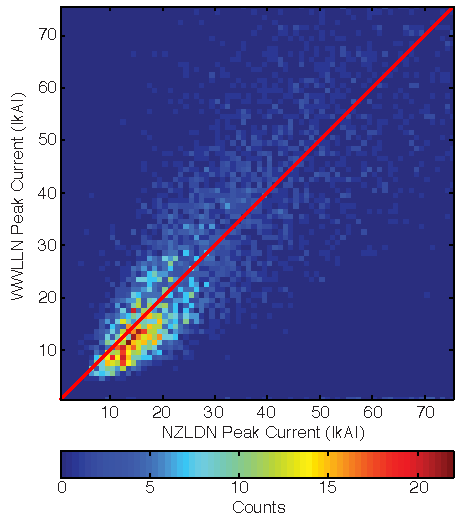
\includegraphics[width=19pc,angle=0]{energy/Figures/PPS_PvI_Error.pdf}\\
 \caption{WWLLN peak current versus NZLDN return stroke peak current for three time periods in 2009 using 5260 matches. WWLLN peak current derived from $P_{stroke} = 1676 * I_{peak}^{1.62}$, 84\% of strokes are within range of the unity line (red solid line) with uncertainty taken into account. 86.5\% of NZLDN-WWLLN matched strokes shown (others out of range).}
 \label{energy:fig:pvi}
 \end{figure}

\subsection{Error and Uncertainty}

The model used in relating the stroke power to the peak current uses the 2010 average stroke uncertainty of 17\% from the median of the MAD distribution of all strokes in the year.
If a stroke has an uncertainty greater than 100\% that value is thrown out, doing so only decreases the number of stroke powers by 3.03\%.

The largest source of uncertainty in the calculations arises from the assumptions that are made using the LWPC code and in the calibration process.
The lookup tables used to calculate attenuation on a given stroke are gridded into $5^{\circ}$ by $5^{\circ}$ bins and averaged over the 8-18 kHz frequency range.
This assumes that the attenuation rates do not vary greatly within a given grid and that the frequency spectra of a sferic is relatively flat within the band considered.
The ionospheric models used within the code assume a perfectly smooth day or night ionosphere, paths crossing the terminator are weighted averages of these values.
These issues arise from the inherent speed limitations of the LWPC code.

A secondary source of uncertainty manifests as variations in the WWLLN station calibration factors.
These are not caused by drift in the electronics, rather from variations in the local station environment and the ionosphere along the path.
Local weather could change the gain at a station (for example through water or ice on an antenna) or if there are significant changes in conductivity of the ground or ionosphere.
Since the LWPC code results are fixed, the only free variable in the bootstrapping process are the station conversion factors, so variations in the propagation path manifests within the these factors.
These uncertainties are mitigated by performing a seven day running average of the calibration values but they are still present as daily variations in the calibrations.

Uncertainties that arise through the use of the LWPC model and through the station calibrations are seen through the MAD of each stroke.
Without these uncertainties each stations should agree on the detected stroke power, however the variations between each station, due to changes in the propagation path or in the calibration, appear as differences in reported stroke power.
Even with these differences the overall 17\% uncertainty of the WWLLN power measurements is comparable to the 13\% uncertainty in the peak current measurements of the U.S. National Lightning Detection Network (NLDN) \citep{Nag2011}.

\subsection{Comparison to Literature}

The current method of measuring stroke powers using WWLLN results in a consistent global median RMS power of 1.0 x $10^6$~W for 2010.
However it has been shown in past literature on radiated stroke power that the average is between $3\pm4$ x $10^9$~W and  $2\pm2$ x $10^{10}$~W \citep{Krider1983}.
A gain of 35 dB to 43 dB in power is needed to bring the WWLLN stroke powers into the range of those in the literature.
Three aspects of our measurement technique: peak vs RMS power, digital filtering, and the attenuation of the ground and sky wave near the stroke combine to explain this large difference in the scalable value of the reported stroke power.

The analysis of the difference was done using the raw waveform data from three stations: the secondary Seattle station, the Canaveral station and the Tallahassee station.
Data was taken from between 20 April 2011 and 9 May 2011. In this interval 198 events were selected that had a clear waveform at the network trigger time.

All of the measurements of power in the literature are measurements of peak power, however WWLLN is measuring RMS power.
The average peak value of the sferic waveform is 8.8 dB greater than the RMS value of the waveform. 

Before the power value is computed at a WWLLN station the full waveform is sent through a 6 to 18 kHz 16 point FIR bandpass filter.
This filter is used to cut out the strong signals from various high powered VLF communications transmitters.
While most of the VLF radiated power is in the 6 to 18 kHz band, it is not a sharp cutoff.
This filtering of the waveform before calculating power causes a power reduction of 1.5 dB.

The biggest effect on the received stroke power is caused by the distances involved in the measurement and most particularly the differences between the ground and sky wave near the stroke and the waveguide propagated signal (and hence received powers).
Most of the VLF power measurements in the literature have measured waveforms at around 100km from the stroke.
These distances are near enough that the ground and sky wave has not yet been attenuated by the structure of the Earth-ionosphere waveguide.

To measure the effect that the nearby high attenuation will have compared to a signal in the waveguide the difference in stroke power of the VLF transmitter near Seattle, NLK (250 kW radiated power at a frequency of 24.8 kHz, i.e. \citet{Clilverd2009}), was compared to the same signal seen at two stations in Florida.
A second transmitter in Hawaii, NPM (500 kW radiated power at a frequency of 21.4 kHz), was used as a reference for both stations.
The two Florida stations were chosen as they are far from both VLF transmitters and sample at a Nyquist frequency of 48kHz, well above the frequencies of the lightning peak power and the VLF radio transmitter frequencies.

The LWPC code estimate for the transmitter signal at the WWLLN stations is compared to the measured transmitter signal to determine the conversion factor for each event.
The conversions are found to be consistent with calculations and calibrations reported in this study for broadband lightning produced signals.
Based on the verification of the LWPC code performed by \citet{Thomson2010}, LWPC is confidently used as a ground truth for this comparison.

The conversion factors from the NLK and NPM signals present in the selected waveforms were used to calculate the power of the two transmitters using the same method as the WWLLN power calculations.
To determine the importance of the ground wave, the ratio of estimated NLK to NPM powers at Seattle were divided by the NLK to NPM ratio at the two Florida stations.
This ratio is necessary, instead of just the Seattle NLK to actual NLK power ratio, in order to normalize out any intrinsic errors in the calculation process.
Measuring the waveguide signal causes a loss of 17.90 dB to 23.83 dB on the signal power as seen by WWLLN compared to the corresponding nearby ground and sky wave measurements.

These three factors show how 27.95 to 39.21 dB of power is lost from ground wave measurements to those made of the waveguide propagating fields by WWLLN, which is in the range if the 35 to 43 dB loss needed to explain the difference between the WWLLN and past power measurements.

This analysis leads to the conclusion that the power being measured by WWLLN is not the absolute power of the stroke, rather it is the RMS power radiated into the Earth-ionosphere waveguide in the 6-18 kHz band.

\subsection{Power Distribution}

Stroke power in a given thunderstorm, region or time span closely follows a lognormal distribution \citep{Golde1977}. Figure~\ref{energy:fig:distribution} shows the stroke power distribution for all strokes seen by WWLLN in 2010 along with the distributions for the three major chimney regions of the Americas, Africa/Europe and Asia/Australia.
The Americas and Asia/Australia show similar distributions, likely a result of having similar WWLLN coverage, while Africa/Europe differ, possibly due to uneven network coverage.

 \begin{figure}[t]
 \noindent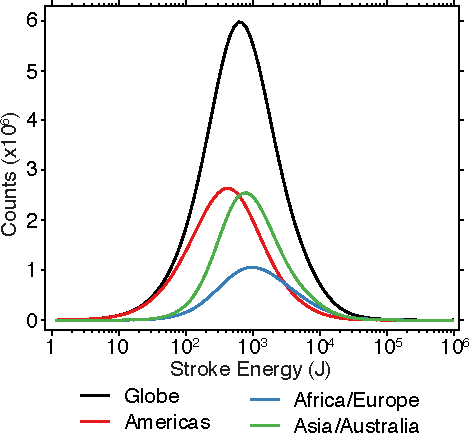
\includegraphics[width=19pc,angle=0]{energy/Figures/PPS_Distribution2.pdf}\\
 \caption{Histogram of stroke powers for 2010 with 100 logarithmically spaced bins, the histogram for the globe (1.4 x 10$^8$ strokes) is shown in black, the Americas (6.1 x 10$^7$ strokes) in blue, Africa/Europe (2.4 x 10$^7$ strokes) in red and Asia/Australia (5.0 x 10$^7$ strokes) in green. Error bars are too small to display.}
 \label{energy:fig:distribution}
 \end{figure}
 
When the power distribution of figure~\ref{energy:fig:distribution} is converted to peak current using equation~\ref{energy:eq:Peq} it can be compared to earlier measurements of peak current distributions.
We can compare the WWLLN peak current distribution to that of \citet{Popolansky1972} as shown in \citet{Golde1977}.
That study used peak current data from 624 return strokes to create a cumulative probability distribution of stroke currents as shown in Figure~\ref{energy:fig:PPS_CDF}.
A similar frequency distribution was created using the WWLLN peak current estimates and is shown in the same figure.
As can be seen, the WWLLN distribution is shifted by a factor of two compared to the previous distribution, which is expected as WWLLN is known to detect higher current strokes when compared to what is seen by regional ground based networks \citep{Abarca2010}.
In a comparison to the NLDN those authors found that the probability distribution function of the WWLLN coincident strokes was similarly of an order two higher than the distribution for all NLDN strokes.
These comparisons further validate the stroke power to peak current relation of equation~\ref{energy:eq:Peq} and demonstrates this relationship is likely valid for the entire global network, and not just the New Zealand region.

\begin{figure}[ht!]
   \centering
   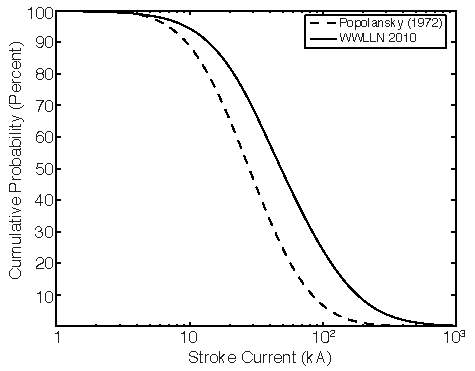
\includegraphics[scale=.6]{energy/Figures/PPS_CDF.pdf}
 \caption{The cumulative probability distributions of stroke current for the best fit of the \citet{Popolansky1972} data (dashed) and the 2010 WWLLN dataset (solid).}
 \label{energy:fig:PPS_CDF}
 \end{figure}

Africa has a lower detection efficiency in the network due to the small number of stations on the continent.
With a lower detection efficiency only the strongest strokes are seen by the more distant stations while the weaker strokes are not seen by these stations due to the stronger attenuation of VLF over continents than for propagation paths over water \citep{Wait1970}.
An initial effort to model the detection efficiency of WWLLN showed this effect very strongly (\citet{Rodger2006}, Fig. 11).
This results in the distribution of figure~\ref{energy:fig:distribution}, with fewer low powered strokes occurring over Africa compared to the other regions.

Without a full understanding of the regional detection efficiency of the network it cannot be concluded if every regions follows the same lognormal power distribution or whether local environments affect the power of strokes in the region.
However, the bootstrap calibration process described in the current study may allow new estimates of the global variation in WWLLN detection efficiency, following \citet{Rodger2006}.

\section{Conclusion}

A new method of measuring the VLF waveguide mode power radiated from lightning using the WWLLN has been shown and validated.
While not the total radiated power of the strokes, the power measured is directly related to the peak current and therefore to inherent properties of the strokes.
Our study shows that WWLLN observations can provide realistic return stroke peak current measurements in addition to the timing and location of global lightning activity.

An enhanced WWLLN allows for a global real time view of lightning with the ability to distinguish between weak and strong strokes.
This will allow for future research into areas such as the long range evolution of thunderstorms over oceans, wider surveys of terrestrial gamma ray flashes, and with a more complete understanding of detection efficiency an analysis of global lightning power output.

\section{acknowledgment} 
The authors wish to thank the World Wide Lightning Location Network (http://wwlln.net), a collaboration among over 50 universities and institutions, for providing the lightning location data used in this paper.

We are grateful to the New Zealand MetService Ltd. for collecting the NZLDN data, and to Antarctica New Zealand for supporting the operation of the Scott Base WWLLN station.

This research was supported in part by the National Science Foundation Grant \#AGS-0809988.
